% Appendix C

\chapter{Notes on neural networks} % Main appendix title

\label{AppendixA} % For referencing this appendix elsewhere, use \ref{AppendixA}

\section{The building blocks of neural networks}

%\lhead{Appendix C. \emph{Statistical Tests}} % This is for the header on each page - perhaps a shortened title
A good starting point for studying the structure of a neural network is to consider a softmax regression model,

$$\mathbf{f}(\mathbf{x}) = \text{softmax}(\mathbf{W}\mathbf{x} + \mathbf{b})$$

where $\mathbf{W} \in \mathbb{R}^{K \times D}$ are the weights and $\mathbf{b} \in \mathbb{R}^{K \times 1}$ (sometimes incorporated into into the weights via the bias trick) and $\text{softmax}(x) = \frac{\exp(x)}{\sum_{x'}\exp(x)}$ generalises the sigma logistic function. The softmax gives us a vector of $K$ probabilities $\mathbf{p}_i \in \mathbb{R}^{K \times 1}$ for each input sample $\mathbf{x}_i$. The loss function $L = \frac{1}{N}\sum_{i=1}^N L_i$ where $L_i = D_{KL}(\mathbf{p}_i || p(y_i))$. Given the ground truth $y_i$ puts all probability mass on one value, the divergence term reduces to $L_i = -\log(p_{y_i})$. Now, for a given \emph{score}, $s_k = \mathbf{w}_k^T\mathbf{x} + b_k$, its gradient is given by, $\frac{\partial L_i}{\partial s_k} = -\frac{1}{p_{y_i}}\cdot\frac{\partial p_{y_i}}{\partial s_k}$. For $k = y_{i}$, $$\frac{\partial p_{y_i}}{\partial s_k}
= \frac{\partial}{\partial s_k}\frac{e^{s_{y_i}}}{\sum_j e^{s_j}}
= p_{y_i} - p_{y_i}^2 \implies \frac{\partial L_i}{\partial s_k}
= p_{y_i} - 1$$
For $k \neq y_{i}$, $$\frac{\partial p_{k}}{\partial s_k}
= -p_kp_{y_i} \implies \frac{\partial L_i}{\partial s_k} = p_k$$
Hence, in general, $$\frac{\partial L_i}{\partial s_k}
= p_k - 1(k = y_i)$$

Now, to construct a true neural network, we introduce an intermediate \emph{hidden} layer separating the input from the output,

\begin{align}
\mathbf{h}(\mathbf{x}) &= \sigma(\mathbf{W}^{(1)}\mathbf{x}  + \mathbf{b}^{(1)}) & \text{(hidden layer)} \notag \\
\mathbf{f}(\mathbf{x}) &= \text{softmax}(\mathbf{W}^{(2)}\mathbf{h} + \mathbf{b}^{(2)}) & \text{(output layer)}\notag
\end{align}

This hidden layer creates an intermediate representation of the input data. The essence of \emph{deep learning} is to model a hierarchy of multiple representations. Neural networks are therefore apt as a deep learning framework as, indeed, we may extend to a multi-layer network simply by stacking a desired layers,

$$\mathbf{f}(\mathbf{x}) = \sigma(\mathbf{W}^{(M)}\sigma(\mathbf{W}^{(M-1)}(\cdots\sigma(\mathbf{W}^{(1)}\mathbf{x} + \mathbf{b}^{(1)})\cdots)  + \mathbf{b}^{(M-1)})  + \mathbf{b}^{(M)})$$

A neural network may be used for classification and regression, the output passed through mean-squared error in the latter case. Despite the complexity, this model can be trained with standard gradient descent techniques. Despite an elongated history, feed-forward neural networks and their variants have seen a resurgence of popularity in recent years, with the advent of deep learning. Neural networks are very powerful non-linear models, which are in fact capable of fitting any smooth function given enough layers, making them \emph{universal approximaters}. A simple example of a neural network fitting an absolute value function is given in Figure \ref{fig:universalapproximater}.

%\begin{figure}
%\centering
%\begin{tabular}{cc}
%\subfloat[]{\includegraphics[width=0.49\textwidth]{Figures/universalapproximater.pdf}} & 
%\subfloat[]{\includegraphics[width=0.5\textwidth]{Figures/sgd.pdf}}
% \end{tabular}
% \caption{A simple example of a neural network fitting an absolute value function (A) and the corresponding learning curve for stochastic gradient descent (B). Generated with \texttt{mlpDemo.m}.}
% \label{fig:universalapproximater}
% \end{figure}

Note that we endow each hidden layer with its own set of weights. Though a neural network in non-linear and not convex, it remains differentiable and therefore trainable with gradient descent. The procedure for computing the gradients at each iteration of a gradient descent is called backpropagation. Backpropagation is an application of the chain rule to the graph structure of model. The crucial formula for backpropagation, as presented in the 1986 paper of Rumelhart, Hinton, and Williams is,

$$\frac{\partial L}{\partial x_i} = \sum_j \frac{\partial L}{\partial y_i} w_{ij}$$

NEED TO PUT THE FIRST PRINCIPLES DERIVATION FOR BACKPROP

where the gradient of the score $x_i$ at a given layer is the sum product of the gradients of the activations $y_j$ emanating from it and the weights $w_{ij}$ between them. From a practical standpoint, each layer $l$ over which we perform backpropagation requires three computations:

\begin{enumerate}
\item $\frac{\partial L}{\partial \mathbf{s}^{(l)}}$, the gradient of the \emph{scores}, $\mathbf{s}^{(l)} = \mathbf{W}^{(l)}\mathbf{x}^{(l)} + \mathbf{b}^{(l)}$.
\item $\frac{\partial L}{\partial \mathbf{W}^{(l)}}$, the gradient of the weights. All weights are subsequently updated to make the descent step.
\item $\frac{\partial L}{\partial \mathbf{x}^{(l)}}$, the gradient of the input (previous activation). This is the \emph{error signal} that is passed back to the layer below.
\end{enumerate}

Let us first consider (1), the gradient of the scores. We previously derived the gradient for the particular case of an output layer. In general, we compute, $\frac{\partial L}{\partial \mathbf{s}^{(l)}} = \frac{\partial L}{\partial \boldsymbol\sigma^{(l)}}\cdot\frac{\partial\boldsymbol\sigma^{(l)}}{\partial\mathbf{s}^{(l)}}$ where $\frac{\partial L}{\partial \boldsymbol\sigma^{(l)}} = \frac{\partial L}{\partial \mathbf{x}^{(l+1)}}$, since the present activation and the following input are one in the same. The activation function $\sigma$, applied element-wise, is classically the sigmoid function or else the hyperbolic tangent function (itself a linear transformation of sigmoid), and nowadays more commonly the rectified linear unit (ReLU) function and its variants. Since we have $\sigma(\mathbf{s}) = [\sigma(s_1), \sigma(s_2), \cdots \sigma(s_k)]^T$, an element-wise transformation, we can calculate the gradient element-wise as,

$$
\frac{\partial L}{\partial \mathbf{s}^{(l)}} =
\begin{bmatrix}
\frac{\partial L}{\partial\sigma_1^{(l)}}\cdot\frac{\partial\sigma_1^{(l)}}{\partial{s}_1^{(l)}} \\ 
\vdots \\
\frac{\partial L}{\partial\sigma_k^{(l)}}\cdot\frac{\partial\sigma_k^{(l)}}{\partial{s}_k^{(l)}} \\
\end{bmatrix},
$$

where for sigmoid, $\frac{\partial\sigma_i^{(l)}}{\partial{s}_i^{(l)}} = \partial\sigma_i^{(l)}(1 - \sigma_i^{(l)})$, and for ReLU, $\frac{\partial\sigma_i^{(l)}}{\partial{s}_i^{(l)}} = 1_{\{\sigma_i^{(l)} > 0\}}$.

For computation (2), the weights gradient, consider, $\frac{\partial L}{\partial w_{kj}^{(l)}} = \frac{\partial L}{\partial s_j}\cdot\frac{\partial s_j}{\partial w_{kj}^{(l)}} = \frac{\partial L}{\partial s_j}\cdot x_j$. In vector form this gives us, $\frac{\partial L}{\partial \mathbf{s}^{(l)}}\mathbf{x}^T$, that is, the outer product of the score gradient and the input vector. Considering that the loss over a batch is the sum of losses for each sample, we have in general, for batch $\mathbf{X} \in \mathbb{R}^{D \times M}$,

$$\frac{\partial L}{\partial \mathbf{W}^{(l)}} = \frac{\partial L}{\partial \mathbf{s}^{(l)}}\cdot\mathbf{X}^T$$

For the bias terms, consider that with the bias trick, the gradients $\frac{\partial s_j}{\partial b_{k}^{(l)}} = 1, \forall k$. We can therefore simply sum the score gradients over the size $m$ batch, $\sum_m\frac{\partial s_{mj}}{\partial b_{k}^{(l)}}$. 

Finally, for computation (3), simply consider the chain rule, $\frac{\partial L}{\partial\mathbf{x}^{(l)}} = \frac{\partial L}{\partial\mathbf{s}^{(l)}}\cdot\frac{\partial\mathbf{s}^{(l)}}{\partial\mathbf{x}^{(l)}}.$ It is easy to show by forming the Jacobian matrix that $\frac{\partial\mathbf{s}^{(l)}}{\partial\mathbf{x}^{(l)}} = \mathbf{W}^{(l)}$. Hence,

$$\frac{\partial L}{\partial \mathbf{x}^{(l)}} = \frac{\partial L}{\partial \mathbf{s}^{(l)}}\cdot\mathbf{W}^T$$

This final gradient is passed to the previous layer as $\frac{\partial L}{\partial \boldsymbol{\sigma}^{(l-1)}}$ to continue the backpropagation.

\subsection{Convolutional neural networks}

In the field of image analysis, the mask (or filter, or kernel) is an important construct. A \emph{convolution} is an operation involving an initial image and the mask. The operation is equivalent to flipping the mask both vertically and horizontally and then visually placing the it over each pixel in turn. The output is the sum over a pixel-wise product of the mask and the sub-image. Masks are usually symmetric, so flipping is unnecessary. Recall from signal processing, the \emph{convolution} between two functions,

$$(f * g)(t) \triangleq \int_{-\infty}^{+\infty}f(\tau)g(t-\tau)d\tau$$

In image processing, a convolution between an image $\mathbf{I}$ and \emph{kernel} $\mathbf{K}$ of size $d \times d$ and centered at a given pixel $(x, y)$ is defined as,

$$(\mathbf{I} * \mathbf{K})(x, y) = \sum_{i = 1}^{d}\sum_{j = 1}^{d} \mathbf{I}(x + i -d/2, y + j - d/2) \times \mathbf{K}(i, j)$$

Convolutional neural networks are a family of neural network architectures having at least one convolutional layer. \emph{LeNet} is the original CNN network architecture, bearing the name of Yann Lecun, who proposed it in the 90s. Its architecture can be written,

\begin{align}
\mathbf{H}_1 &= \sigma(\mathbf{X} * \mathbf{K}^{(1)}) & \text{(first convolutional layer)}\notag \\
\mathbf{P}_1 &= \text{maxpool}(\mathbf{H}_1) & \text{(first pooling layer)}\notag \\
\mathbf{H}_2 &= \sigma(\mathbf{P}_1 * \mathbf{K}^{(2)}) & \text{(second convolutional layer)} \notag \\
\mathbf{P}_2 &= \text{maxpool}(\mathbf{H}_2) & \text{(second pooling layer)} \notag \\
\mathbf{F}_1 &= \sigma(\mathbf{W}^{(1)}\mathbf{P}_2 + \mathbf{b}^{(1)}) & \text{(first fully-connected layer)} \notag \\
\mathbf{F}_2 &= \sigma(\mathbf{W}^{(2)}\mathbf{F}_1 + \mathbf{b}^{(2)}) & \text{(second fully-connected layer)} \notag \\
\mathbf{f}(\mathbf{X}) &= \text{softmax}(\mathbf{W}^{(3)}\mathbf{F}_2 + \mathbf{b}^{(3)}) & \text{(output layer)} \notag
\end{align}

Convolutional Neural Networks (CNNs) are the current state-of-the-art in many computer vision tasks. Their great success in image classification\footnote{See ImageNet Large Scale Visual Recognition Competition (LSVRC), 2012 (\cite{krizhevsky2012imagenet}).} heralded a resurgence of interest in neural networks and deep learning. CNNs make the specific assumption of receiving image inputs and emulate the process of feature extraction using image masks. It has been found that using a pre-trained CNN as a general-purpose feature extractor for a simple linear model can yield significant improvements over even the most meticulously hand-crafted feature engineering (\cite{sharif2014cnn}). Another possibility is to use the pre-trained weights as an initialisation for training on a new dataset. Both are examples of transfer learning.

The cornerstone of the CNN is the \emph{convolutional layer}, a hidden layer where a square grid of weights is convolved with the input, just like an image mask (now, however, the mask is learned as part of an all-encompassing model). The output of the convolutional layer is akin to a convolved image. Next, the non-linear activation function, ReLu (REctified Linear Unit), is applied to zero-out any negative values. Next there is a \emph{pooling} layer, emulating \emph{downsampling}. Here, each group of (usually) four values (pixels) is replaced by the maximum (sometimes the mean) of the four, leaving a single most intense pixel. This pooling method is known as \emph{max pooling}. This sequence of \texttt{CONV->RELU->POOL} layers may be repeated multiple times to create a deep architecture. Finally, a few fully-connected layers round off the architecture. Though it seems far more sophisticated than a MLP, it can be shown that a CNN can be represented as a classical fully-connected neural network. For example, a convolutional layer can be represented as a sparse fully-connected layer. Various techniques have been developed for training these vast models, for example momentum optimisers, weight initialisation, batch normalisation\footnote{Batch normalisation mitigates \emph{internal covariate shift}, the fluctuations to the internal distributions of activations that make convergence so arduous.}, and \emph{dropout}\footnote{Dropout involves deactivating (setting to $0$) hidden units in fully-connected layers according to a Bernoulli probability. This is repeated for every forward-backward pass of the network, such that every training example is trained on a different sub-graph of the network.} for regularisation.

\subsubsection{Backprop through Convolutional Layers}

But how do we compute the gradient for the convolutional kernel? Let us consider the following simple convolution,

$$
\underbrace{\begin{bmatrix}
x_{11} & x_{12} & x_{13} \\
x_{21} & x_{22} & x_{23} \\
x_{31} & x_{32} & x_{33} \\
\end{bmatrix}}_{\mathbf{X}} * 
\underbrace{\begin{bmatrix}
k_{11} & k_{12} \\
k_{21} & k_{22} \\
\end{bmatrix}}_{\mathbf{K}} =
\underbrace{\begin{bmatrix}
s_{11} & s_{12} \\
s_{21} & s_{22} \\
\end{bmatrix}}_{\mathbf{S}}
$$

This gives the set of equations,

\begin{align}
s_{11} &= k_{11}x_{11} + k_{12}x_{12} + k_{21}x_{21} + k_{22}x_{22}\notag \\
s_{12} &= k_{11}x_{12} + k_{12}x_{13} + k_{21}x_{22} + k_{22}x_{23}\notag \\
s_{21} &= k_{11}x_{21} + k_{12}x_{22} + k_{21}x_{31} + k_{22}x_{32}\notag \\
s_{22} &= k_{11}x_{22} + k_{12}x_{23} + k_{21}x_{32} + k_{22}x_{33}\notag
\end{align}

The partial derivatives of the kernel's elements are therefore,

\begin{align}
\frac{\partial{L}}{\partial{k_{11}}} &= \frac{\partial{L}}{\partial{s_{11}}}x_{11} + \frac{\partial{L}}{\partial{s_{12}}}x_{12} + \frac{\partial{L}}{\partial{s_{21}}}x_{21} + \frac{\partial{L}}{\partial{s_{22}}}x_{22}\notag \\
\frac{\partial{L}}{\partial{k_{12}}} &= \frac{\partial{L}}{\partial{s_{11}}}x_{12} + \frac{\partial{L}}{\partial{s_{12}}}x_{13} + \frac{\partial{L}}{\partial{s_{21}}}x_{22} + \frac{\partial{L}}{\partial{s_{22}}}x_{23}\notag \\
\frac{\partial{L}}{\partial{k_{21}}} &= \frac{\partial{L}}{\partial{s_{11}}}x_{21} + \frac{\partial{L}}{\partial{s_{12}}}x_{22} + \frac{\partial{L}}{\partial{s_{21}}}x_{31} + \frac{\partial{L}}{\partial{s_{22}}}x_{32}\notag \\
\frac{\partial{L}}{\partial{k_{22}}} &= \frac{\partial{L}}{\partial{s_{11}}}x_{22} + \frac{\partial{L}}{\partial{s_{12}}}x_{23} + \frac{\partial{L}}{\partial{s_{21}}}x_{32} + \frac{\partial{L}}{\partial{s_{22}}}x_{33}\notag
\end{align}

It is evident that the kernel derivative is simply a convolution between the score ``image'' $\mathbf{S}$ and the input,

$$
\underbrace{\begin{bmatrix}
\frac{\partial{L}}{\partial{k_{11}}} & \frac{\partial{L}}{\partial{k_{12}}} \\
\frac{\partial{L}}{\partial{k_{21}}} & \frac{\partial{L}}{\partial{k_{22}}} \\
\end{bmatrix}}_{\frac{\partial L}{\partial\mathbf{K}}}
=
\underbrace{\begin{bmatrix}
x_{11} & x_{12} & x_{13} \\
x_{21} & x_{22} & x_{23} \\
x_{31} & x_{32} & x_{33} \\
\end{bmatrix}}_{\mathbf{X}} *
\underbrace{\begin{bmatrix}
\frac{\partial{L}}{\partial{s_{11}}} & \frac{\partial{L}}{\partial{s_{12}}} \\
\frac{\partial{L}}{\partial{s_{21}}} & \frac{\partial{L}}{\partial{s_{22}}} \\
\end{bmatrix}}_{\frac{\partial L}{\partial\mathbf{Y}}}
$$

By following a similar procedure for the input gradient, it is easy to see that,

$$\frac{\partial L}{\partial \mathbf{X}^{(l)}} = \frac{\partial L}{\partial \mathbf{S}^{(l)}} * \text{rot180}\big(\mathbf{K}\big),$$

that is, the input gradient is (almost shockingly) equal to a convolution between the (zero-padded) scores gradient and a $180^{\circ}$ rotation of the kernel matrix. To elucidate this somewhat, consider again that the convolution operation may be represented as a matrix operation, by stacking a flattened kernel at offsets and flattening the input image to a vector. Thus, our kernel matrix becomes,

$$
\underbrace{\begin{bmatrix}
k_{11} & k_{12} & 0 & k_{21} & k_{22} & 0 & 0 & 0 & 0 \\
0 & k_{11} & k_{12} & 0 & k_{21} & k_{22} & 0 & 0 & 0 \\
0 & 0 & 0 & k_{11} & k_{12} & 0 & k_{21} & k_{22} & 0 \\
0 & 0 & 0 & 0 & k_{11} & k_{12} & 0 & k_{21} & k_{22} \\
\end{bmatrix}}_{\mathbf{K}}
\underbrace{\begin{bmatrix}
x_{11} \\
x_{12} \\
x_{13} \\
x_{21} \\
x_{22} \\
x_{23} \\
x_{31} \\
x_{32} \\
x_{33} \\
\end{bmatrix}}_{\mathbf{X}} =
\underbrace{\begin{bmatrix}
s_{11} \\
s_{12} \\
s_{21} \\
s_{22} \\
\end{bmatrix}}_{\mathbf{S}}
$$

Now, in the feed-forward setting, the gradient of the input is computed as the matrix product of the gradient of the loss, and the transpose of the weight matrix. It can be seen easily that a transposition of this sparse kernel matrix amounts to the half rotation of the kernel in a convolution operation.

\subsubsection{Backprop through max pooling layers}

Finally, consider the gradient for max pooling. We treat this similar to differentiating the ReLU activation function. If we have, for example, a $2 \times 2$ block of neurons $\boldsymbol\sigma=\{\sigma_1, \sigma_2, \sigma_3, \sigma_4\}$, then for pooling function $p$, we have $\frac{\partial{L}}{\partial{\sigma_i}} = \frac{\partial{L}}{\partial{p(\boldsymbol\sigma)}}\cdot\frac{\partial{p(\boldsymbol\sigma)}}{\partial{\sigma_i}}$, where $\frac{\partial{p(\boldsymbol\sigma)}}{\partial{\sigma_i}} = 1_{\{\sigma_1 = \max(\boldsymbol\sigma)\}}$.

\subsubsection{Transposed convolutional layers}

Transposed convolutional layers (sometimes incorrectly called \emph{deconvolutional layers}\footnote{Formally speaking, a deconvolution inverts a convolution. Transposed convolutional layers cannot be said to do this.}) play an essential role in networks where the compressed hidden layers are eventually \emph{decompressed}, usually to the original input sizes. Examples of such networks are convolutional autoencoders, fully-convolutional networks for segmentation, and the generator networks of GANs. A deconvolution computation is similar to that of the convolutional gradient--they are implemented as a ``convolutional transpose''--specifically, a convolution between the layer input and the rotation of the kernel. The gradient of a transposed convolutional layer is therefore a normal convolution between the gradient of the scores and the kernel.

Recall that convolutional layers may be used for downsampling (rather than a pooling layer) when the stride $s > 1$. Likewise, the convolutional transpose will \emph{upsample} its inputs, back towards the original input size. In this case we have what is called \emph{fractional stride} $1/s$. To see this, take the convolution of stride 2,

$$
\underbrace{\begin{bmatrix}
x_{11} & x_{12} & x_{13} & x_{14} \\
x_{21} & x_{22} & x_{23} & x_{24} \\
x_{31} & x_{32} & x_{33} & x_{34} \\
x_{41} & x_{42} & x_{43} & x_{44} \\
\end{bmatrix}}_{\mathbf{X}} * 
\underbrace{\begin{bmatrix}
k_{11} & k_{12} \\
k_{21} & k_{22} \\
\end{bmatrix}}_{\mathbf{K}} =
\underbrace{\begin{bmatrix}
s_{11} & s_{12} \\
s_{21} & s_{22} \\
\end{bmatrix}}_{\mathbf{S}}
$$

The corresponding sparse kernel matrix is,

\setcounter{MaxMatrixCols}{20}

$$
\begin{bmatrix}
k_{11} & k_{12} & 0 & 0 & k_{21} & k_{22} & 0 & 0 & 0 & 0 & 0 & 0 & 0 & 0 & 0 & 0 \\
0 & 0 & k_{11} & k_{12} & 0 & 0 & k_{21} & k_{22} & 0 & 0 & 0 & 0 & 0 & 0 & 0 & 0 \\
0 & 0 & 0 & 0 & 0 & 0 & 0 & 0 & k_{11} & k_{12} & 0 & 0 & k_{21} & k_{22} & 0 & 0 \\
0 & 0 & 0 & 0 & 0 & 0 & 0 & 0 & 0 & 0 & k_{11} & k_{12} & 0 & 0 & k_{21} & k_{22} \\
\end{bmatrix}
$$

It can be seen that the transpose of this matrix, multiplied by the flattened scores gradient, $\frac{\partial L}{\partial \mathbf{s}^{(l)}}$, is equivalent to the convolution,

$$\frac{\partial L}{\partial \mathbf{X}}=
\underbrace{\begin{bmatrix}
0 & 0 & 0 & 0 & 0 \\
0 & s_{11}' & 0 & s_{12}' & 0 \\
0 & 0 & 0 & 0 & 0 \\
0 & s_{21}' & 0 & s_{22}' & 0 \\
0 & 0 & 0 & 0 & 0 \\
\end{bmatrix}}_{\frac{\partial L}{\partial \mathbf{S}}} * 
\underbrace{\begin{bmatrix}
k_{22} & k_{21} \\
k_{12} & k_{11} \\
\end{bmatrix}}_{\text{rot180}(\mathbf{K})}
$$

which we can refer to as having $s = 1/2$. It has been shown that the transposed convolutional layers found in GANs and other models tend to an undesirable ``checkerboard'' effect in the image output. A simple workaround appears to be upsampling followed by a standard convolution\footnote{https://distill.pub/2016/deconv-checkerboard/}.

\subsubsection{Upsampling layers}

While transposed convolutional layers have weights making them \emph{learnable} upsampling layers, static forms of upsampling are used in convolutional networks too. One example is \emph{bilinear interpolation}. It can easily be seen on paper that, for a fixed, integral-sized interpolation, this is equivalent to a fixed convolution applied with fractional stride. For example, a bilinear upsampling by a factor of $2$ is equivalent to convolving the input with the kernel,

$$
\begin{bmatrix}
1/4 & 1/2 & 1/4 \\
1/2 & 1 & 1/2 \\
1/4 & 1/2 & 1/4 \\
\end{bmatrix}
$$

with a stride of $1/2$. Likewise, a nearest neighbour upsampling can be achieved by running a $2 \times 2$ convolution with $1/2$ stride.


\section{A brief history of deep image classifiers}
\ref{sec:brief_history_classifiers}
In the following we sketch out a short overview of the advancement of convolutional neural networks (CNNs) from minority success to the predominant analysis tool in computer vision.

\subsection{LeNet}

The earliest recognisable CNN is LeNet (\cite{lecun1998gradient}). LeNet is perennially associated with MNIST, the dataset it was developed to classify. MNIST is a 10-class image dataset of small ($28\times28$px) handwritten digits ($0-9$) in greyscale, crowd-sourced from US school students. For fundamental research in particular, MNIST remains a widely used resource (\cite{sabour2017dynamic}).

%$\mathbf{F}_1 \in \mathbb{R}^{120}$ concatenates the 16 activation maps of size $5\times5$ vector. The rest of the network is like a traditional fully-connected network with $\mathbf{F}_2 \in \mathbb{R}^{84}$ and a $10 \times 1$ output layer.

%* Note that the reduction in size after each convolution is due to convolutions not being performed at the borders (aka *valid* convolution). It is, however, more common to *pad* the input images with zeros to allow convolution on every pixel, thereby preserving the input size. In our model, we have $28 \times 28$ inputs that will be zero-padded.

Datasets of similar resolution to MNIST, albeit in full RGB colour, are CIFAR10 (10 object classes) and CIFAR100 (100 object classes). These datasets tend to pose more of a challenge to object classifiers. For an example of training a deep network on these datasets, see \hyperref[https://github.com/jcboyd/vgg-fun]{https://github.com/jcboyd/vgg-fun}. Despite successes on isolated problems such as in \cite{matan1992reading}, the contemporary hardware was not powerful enough to drive neural networks to their full potential, and interest in them soon declined. Thus followed a second neural network winter\footnote{The first such winter occurred in the 1970s with the publication of ``Perceptrons'' by Minsky and Papert. This was a damning repudiation of the simple Perceptron networks designed by Frank Rosenblatt in 1957.} as researchers turned to models with more rigorous mathematical grounding, such as support vector machines. Nevertheless, the tenacity of deep learning to outperforms its competitors, particularly on image data, won it a minority of champions and defenders (see for example \cite{simard2003best}).

\subsection{AlexNet}

The emphatic victory of AlexNet (\cite{krizhevsky2012imagenet}) in the 2012 ImageNet Large Scale Visual Recognition Challenge (ILSVRC)\footnote{1000 classes, 1 million images} heralded the inexorable rise of CNNs. While emulating the same basic design as LeNet, the AlexNet architecture was deeper (more layers) and wider (more neurons/kernels), and processed larger images ($224\times224\times3$px), featuring in excess of $60$ million parameters over 8 learnable layers. The breakthrough of AlexNet is often attributed to the conjunction of three technological developments:

\begin{enumerate}
\item The rise of graphical processing units (GPUs)
\item The sourcing of large image datasets such as ImageNet
\item The streamlining of neural network training e.g. more stable activation functions (ReLU), adaptive optimisers, regularisers such as dropout, and better weight initialisation or pre-training strategies.
\end{enumerate}

With academic and industrial vision research in full swing, VGGNet\footnote{Visual Geometry Group at Oxford University.} and GoogLeNet were followed as ILSVRC 2014 frontrunners, pushing the state-of-the-art ever further, while achieving lasting fame. The competition winner, GoogLeNet, pioneered a more complex neural network design by engineering the \emph{inception module}, a concatenation of differently-sized convolutions. Laying several inception blocks end-to-end constitutes the 22-learnable-layer GoogLeNet. VGGNet likewise strived for unprecedented network depth (up to 19 learnable layers) while advocating some simple design principles. For example, (padded) $3\times 3$ convolutions are used everywhere, given that a stack of three $3 \times 3$ convolutions with $C$ channels has a receptive field of size $7 \times 7$ on its inputs, despite having $27C^2$ weights, fewer than a single $7 \times 7$ kernel at $49C^2$.

A multitude of network architectures have since been proposed. Among the most influential is ResNet, which introduced the residual block: a skip connection bypassing a stack convolutions. The motivation is to prevent the gradients of deeper layers from overwhelming all others early during training. The residual block thus facilitated the training of extremely deep networks of up to 1202 layers\footnote{However, the standard depths are 50, 101, and 152 layers.}. More recently, EfficientNet proposed a ``compound scaling'' design strategy to increase network depth, width, and resolution in unison to maximise the performance benefit. As of February 2020, the state-of-the-art in ImageNet is an EfficientNet variant. Table \ref{table:convnets} displays results from the history of the ILSVRC challenge illustrating the advancement of minimisation of test error over time. Note that AlexNet was evaluated on the ILSVRC 2012 dataset, whereas all others where evaluated on a similar dataset from the 2014 competition. Also, while GoogLeNet was the ILSVRC 2014 challenge winner, it prevailed only with a complex ensemble approach; we provide single-model results only. 

\begin{table}
\centering
\begin{tabular}{ |c|c|c|c|c| } 
\hline
 Model & Year &  Top-1 & Top-5 & No. Parameters \\ 
 \hline
 AlexNet & $2012$ & $40.7\%$ & $18.2\%$ & $60$M \\
 GoogLeNet & $2014$ & - & $10.1\%$ & $6.8$M\\
 VGG-19 & $2014$ & $25.5\%$ & $8.0\%$ & $144$M \\
 ResNet-152 & $2015$ & $22.2\%$ & $6.2\%$ & $60$M \\
 EfficientNet & 2019 & $15.6\%$ & $2.9\%$ & $66$M \\
 \hline
\end{tabular}
\caption{Single-model test errors on ImageNet for five groundbreaking CNNs. Note AlexNet was evaluated on the ILSVRC 2012 dataset, the others on ILSVRC 2014. Human performance has been estimated to be $5\%$ Top-5 error (\cite{karpathy2014learned}).}
\label{table:convnets}
\end{table}

\subsection{ConvNets for semantic segmentation}

Image segmentation may be viewed as a classification problem, sorting pixels into background and foreground classes. It was this conception that led \cite{ciresan2012deep} to apply deep CNNs to segment neuronal membranes in electron microscopy images as a pixel-wise classifier. Despite its accuracy, the sliding-window approach was hopelessly slow and quickly improved upon with fully convolutional networks \cite{long2015fully}. Such networks were designed for image-to-image translation, inputting an input image, and outputting a segmentation image. This was done by removing the fully-connected layers from a CNN classifier and replacing them with additional convolutions and upsampling layers\footnote{Upsampling layers are any of a family of network layers reversing the pooling operation and increasing image resolution.}. The essential property of a network with only convolutional layers is that it may process variable sized inputs. Convolutional layers, which share across space, are agnostic to input size and efficiently emulate a sliding-window process. A refinement of FCNs is U-Net (\cite{ronneberger2015u}), which was first designed for segmenting cells in biomedical imagery, and has since proven an immensely powerful tool for image processing tasks.

\section{A brief history of neural object detection}

\tikzstyle{block} = [rectangle, draw, fill=blue!20, node distance=2.5cm,
    text width=3.5em, text centered, rounded corners, minimum height=3em]
\tikzstyle{line} = [draw, -latex']

An object detection system is a model or automated pipeline that both localises and classifies ontological objects in images. Localisation is usually expressed as a bounding box, which the detector emits along with the class prediction as the tuple,

$$f : \mathbf{x} \to \big\{(x, y, w, h, c)\big\}$$

for image $\mathbf{x}$ where $x, y$ are the coordinates of the bounding box center, and $w, h$ are its width and height. The variable $c$ denotes the class of the detected object. In this setting, a detection is deemed a true positive (TP) when the correct class is predicted with an intersection over union (IoU) bounding box overlap of $\text{IoU} > 0.5$. A false positive (FP) occurs when an object is predicted either wrongly or $\text{IoU} < 0.5$, that is \emph{a detection box where there is nothing}. A false negative (FN) occurs when a ground truth detection goes undetected. The remaining contingency, true negatives (TN), are not usually part of the discussion.

%\begin{figure}[hb]
%\centering
%
%\tikzset{every picture/.style={line width=0.75pt}} %set default line width to 0.75pt        
%
%\begin{tikzpicture}[x=0.75pt,y=0.75pt,yscale=-1,xscale=1]
%%uncomment if require: \path (0,467); %set diagram left start at 0, and has height of 467
%
%%Shape: Circle [id:dp5745969695586605] 
%\draw  [fill={rgb, 255:red, 255; green, 200; blue, 200 }  ,fill opacity=1 ] (51,73) .. controls (51,61.95) and (59.95,53) .. (71,53) .. controls (82.05,53) and (91,61.95) .. (91,73) .. controls (91,84.05) and (82.05,93) .. (71,93) .. controls (59.95,93) and (51,84.05) .. (51,73) -- cycle ;
%
%%Shape: Circle [id:dp7426569927405986] 
%\draw  [fill={rgb, 255:red, 200; green, 200; blue, 255 }  ,fill opacity=1 ] (171,73) .. controls (171,61.95) and (179.95,53) .. (191,53) .. controls (202.05,53) and (211,61.95) .. (211,73) .. controls (211,84.05) and (202.05,93) .. (191,93) .. controls (179.95,93) and (171,84.05) .. (171,73) -- cycle ;
%
%%Shape: Circle [id:dp9252288296430268] 
%\draw  [fill={rgb, 255:red, 255; green, 200; blue, 200 }  ,fill opacity=1 ] (111,73) .. controls (111,61.95) and (119.95,53) .. (131,53) .. controls (142.05,53) and (151,61.95) .. (151,73) .. controls (151,84.05) and (142.05,93) .. (131,93) .. controls (119.95,93) and (111,84.05) .. (111,73) -- cycle ;
%
%%Shape: Circle [id:dp6729025851829732] 
%\draw  [fill={rgb, 255:red, 255; green, 200; blue, 200 }  ,fill opacity=1 ] (231,73) .. controls (231,61.95) and (239.95,53) .. (251,53) .. controls (262.05,53) and (271,61.95) .. (271,73) .. controls (271,84.05) and (262.05,93) .. (251,93) .. controls (239.95,93) and (231,84.05) .. (231,73) -- cycle ;
%
%%Shape: Circle [id:dp41960341449353533] 
%\draw  [fill={rgb, 255:red, 200; green, 200; blue, 255 }  ,fill opacity=1 ] (291,73) .. controls (291,61.95) and (299.95,53) .. (311,53) .. controls (322.05,53) and (331,61.95) .. (331,73) .. controls (331,84.05) and (322.05,93) .. (311,93) .. controls (299.95,93) and (291,84.05) .. (291,73) -- cycle ;
%
%%Shape: Circle [id:dp8282065780886362] 
%\draw  [fill={rgb, 255:red, 200; green, 200; blue, 255 }  ,fill opacity=1 ] (351,73) .. controls (351,61.95) and (359.95,53) .. (371,53) .. controls (382.05,53) and (391,61.95) .. (391,73) .. controls (391,84.05) and (382.05,93) .. (371,93) .. controls (359.95,93) and (351,84.05) .. (351,73) -- cycle ;
%
%%Straight Lines [id:da16760548695080602] 
%\draw  [dash pattern={on 4.5pt off 4.5pt}]  (161,43) -- (160,120) ;
%%Straight Lines [id:da5090385930403043] 
%\draw  [dash pattern={on 4.5pt off 4.5pt}]  (221,43) -- (220,120) ;
%%Straight Lines [id:da4044907060915748] 
%\draw  [dash pattern={on 4.5pt off 4.5pt}]  (281,43) -- (280,120) ;
%%Straight Lines [id:da40386086159021517] 
%\draw    (71,112) -- (369,112) ;
%\draw [shift={(371,112)}, rotate = 180] [color={rgb, 255:red, 0; green, 0; blue, 0 }  ][line width=0.75]    (10.93,-3.29) .. controls (6.95,-1.4) and (3.31,-0.3) .. (0,0) .. controls (3.31,0.3) and (6.95,1.4) .. (10.93,3.29)   ;
%
%% Text Node
%\draw (71,73) node   [align=left] {N};
%% Text Node
%\draw (191,73) node   [align=left] {P};
%% Text Node
%\draw (131,73) node   [align=left] {N};
%% Text Node
%\draw (251,73) node   [align=left] {N};
%% Text Node
%\draw (311,73) node   [align=left] {P};
%% Text Node
%\draw (371,73) node   [align=left] {P};
%% Text Node
%\draw (160,129) node   [align=left] {$\displaystyle \tau _{0}$};
%% Text Node
%\draw (220,129) node   [align=left] {$\displaystyle \tau _{1}$};
%% Text Node
%\draw (280,129) node   [align=left] {$\displaystyle \tau _{2}$};
%% Text Node
%\draw (158,21) node   [align=left] {$\displaystyle \{TN,\ FN\} \ \leftrightarrow \ \{TP,\ FP\}$};
%% Text Node
%\draw (405.5,111) node   [align=left] {$\displaystyle p\ =\ 1$};
%% Text Node
%\draw (35.5,111) node   [align=left] {$\displaystyle p\ =\ 0$};
%
%\end{tikzpicture}
%
%\end{figure}
%
%A precision-recall (PR) curve plots $\text{precision} = \frac{TP}{TP + FP}$ against $\text{recall} = \frac{TP}{TP + FN}$. One generates a PR curve by first ranking test predictions made by the model, according to their probabilities. Now, by varying the decision threshold $t$ from $0$ to $1$, we obtain precision and recall at each threshold. Note that (by definition) predictions with probabilities above the threhsold are either TP and FP, whereas below it they are either TN or FN. Depending only on TP and FN, $\text{recall} = 1$ when $t = 0$ and decreases monotonically as $t \to 1$, whenever a TP becomes a FN. $\text{Precision} = P / (P + N)$ when $t = 0$, then increases for each FP that becomes a TN and decreases for each TP that becomes a FN. This produces a saw-tooth effect in the PR curve, which is sometimes rectified to give the \emph{interpolated} PR curve. The average precision (AP) is then the area under this curve,
%
%$$AP = \int_0^1p(r)dr$$
%
%where $p(r)$ is the precision at recall level $r$. Finally, the mean average precision (mAP) is the AP averaged over all object classes.
%
%\myworries{Does the PR curve not therefore account for class imbalance by marginalising the decision threshold. Testing all possible thresholds is like testing all possible priors.}

Whereas the ILSVRC datasets came to set the gold standard in image classification benchmarks, similarly rich datasets predominate for object detection. The Microsoft Common Objects in COntext (COCO) (\cite{lin2014microsoft}) (80 classes $+$ background) and the PASCAL\footnote{Pattern Analysis, Statistical Modelling and Computational Learning} Visual Object Classes (VOC) challenge (20 classes $+$ background) datasets (\cite{everingham2010pascal}) are the two leading datasets against which state-of-the-art object detection systems are tested. The classes of each dataset encompass a range of categories from animals to machinery to household items. Following the explosion of interest in deep CNNs as image classifiers in 2012, rapid progress was made virtually in parallel for neural object detectors. An early example is \emph{Overfeat} (\cite{sermanet2013overfeat})), appearing in 2013. The basic architecture of Overfeat was an AlexNet, modified as a fully-convolutional model. Replacing fully-connected with convolutional layers frees the network from the constraint of a fixed input size. However, no family of detectors is more celebrated than the R-CNN series, the study of which is to be recommended to the student of deep learning.

\subsubsection{R-CNN}

Regions with CNN features (R-CNN) (\cite{girshick2014rich}) began as a disjoint pipeline consisting of four ordered stages:

\begin{itemize}
\item[1)] region proposal
\item[2)] feature extraction,
\item[3a)] object classification 
\item[3b)] bounding box correction
\end{itemize}

A common choice for 1) was ``selective search'' (\cite{uijlings2013selective}), a greedy algorithm that progressively merges homogeneous regions of an input image, from which derive a large number of bounding box proposals. In the R-CNN framework, this may total $\sim2000$ proposals. Feature extraction (2) is then performed by a pre-trained CNN, producing a ``CNN code'' feature vector for each region. For a large dataset and typical hardware constraints, these are necessarily stored offline before proceeding to the final stages. Stage (3a) consists of a set of linear models (typically SVMs) that perform one-vs-the-rest classification for each object class. These models are trained on the outputs of stage (2). Likewise, in stage (3b), a set of per-class (ridge) regression models are learned to correct the region proposal coordinates $(x, y, w, h)$.

\subsubsection{Fast R-CNN}

In Fast R-CNN (\cite{girshick2015fast}) stages 3a) and 3b) are absorbed into the CNN ``backbone'' of stage 2) as appendages to the feature extractor. Whereas previously, regions were ``warped'' to a standard size and passed through the network as separate entities, now entire images are processed in a single forward pass, and regions are cropped from their relative positions in the activation maps. This yields a substantial reduction in run-time. To satisfy the sizes of the classification and regression layers, the encoded regions are quantised by a generalisation of the max pooling layer, RoIPool,

$$\rho : \{\mathbf{X}, \mathcal{B}\} \to \mathbf{Y}$$

where $\mathbf{X} \in \mathbb{R}^{W \times H \times c}$ is the input image, $\mathbf{Y} \in \mathbb{R}^{K \times w \times h \times c}$ are the $K$ RoIs, resized to $w \times h$ and $\mathcal{B}$ is a list of $K$ bounding boxes for the image.

Note that in Fast R-CNN the region proposal algorithm remains an independent component and becomes the major bottleneck at runtime.

\subsubsection{Faster R-CNN}

Faster R-CNN \cite{ren2015faster} completes the work begun in Fast R-CNN by integrating the region proposal algorithm into the network. To achieve this, a separate region proposal network (RPN) is introduced during training. This network is trained to classify object presence (``objectness'') and bounding box coordinates against a ground truth of RoIs. The RPN can produce outputs these for a set of bounding box templates (``anchors'') modeling different sizes and aspect ratios, for every spatial location. Stages 2) and 3) are handled by a Fast R-CNN as before. With no guarantee of convergence when trained end-to-end, a four-step training procedure is undertaken:

\begin{enumerate}
\item the RPN is initialised with ImageNet weights and trained for region proposal alone
\item the R-CNN is initialised with ImageNet weights and trained on the RPN region proposals
\item the RPN is reinitialised with the Fast R-CNN weights (frozen) and the RoI proposal heads are fine-tuned
\item the heads of the R-CNN are fine-tuned against the updated RPN proposals
\end{enumerate}

The outcome of this procedure is a synchronisation of the shared layers of the RPN and R-CNN. Consequently, at test time, the feature extraction (the bulk of the computation) can be performed for both networks in a single forward pass. Then, the RPN heads produce the RoIs for the image, which are passed to the heads of the R-CNN for detection. The overhead of region proposal is therefore negligible, and Faster R-CNN produces state-of-the-art object detection results more or less at real time.

\subsubsection{Mask R-CNN}

The synthesis of object detection and semantic segmentation is called \emph{instance segmentation}. Here, semantic objects are not only localised and classified, but also segmented as individual entities. This is the accomplishment of Mask R-CNN (\cite{he2017mask}), which extends Faster R-CNN by appending yet another branch for segmentation. In addition, the features are taken from different layers of the blackbone and combined in a \emph{feature pyramid network} (\cite{lin2017feature}), as seen also in RetinaNet (\cite{lin2017focal}). Most other implementation details rest unchanged, except that the RoIPool is replaced with an improved RoIAlign layer, involving a bilinear interpolation\footnote{It can easily be seen that a bilinear interpolation with integral scale is equivalent to a convolution with a constant kernel with fractional stride (the backprop being the transposition of this).}.

%Note that in the pytorch implementations, the images are upsampled to minimum 800 x 800, and grayscale images are triplicated to ensure a depth of 3 (albeit separately normalised). In fact, the triplication is a byproduct of the normalisation operation.

\subsubsection{YOLO}

In YOLO (you only look once) (\cite{redmon2016you}), aims to simplify the R-CNN design, so as to increase speed while maintaining accuracy. The system divides a fixed-size image into a grid, and permits at most one detection per grid cell, choosing from a small number of bounding boxes anchors. This is a substantial simplification over R-CNN and other systems. Evidently, this imposes a limit on the number of detectable objects per image. However, this proves to be a negligible constraint for YOLO. Each anchor predicts a bounding box correction, along with a confidence for the presence of an object, and, separately, a softmax probability for each modeled class. The confidence score ground truth is $p(object) \times IOU$ (intersection over union between ground truth and bounding box). At test time one multiplies the confidence by $p(class|object)$ to obtain $p(class) \times IOU$ (by Bayes rule and because we have $p(object|class) = 1)$.

YOLO was succeeded by YOLOv2 (\cite{redmon2017yolo9000}) and YOLOv3 \cite{redmon2018yolov3}, which in turn introduced various improvements. \cite{redmon2017yolo9000} also showed how YOLO can learn over 9000 object detection classes in a semi-supervised way by supplementary data from the full ImageNet dataset.

\section{Transfer learning}

Transfer learning is a set of solutions for learning problems in which training and test data differ in their marginal distribution, or else that the learning tasks differ between model training and deployment (\cite{pan2009survey}). As such, these problems violate the basic assumption for training supervised models. Transfer learning is done between \emph{domains}. A domain $\mathcal{D}$ consists of a feature space $\mathcal{X}$ and marginal probability distribution on that domain $P(X)$. A learning \emph{task} $\mathcal{T}$ is performed on a domain, itself consisting of a label space $\mathcal{Y}$ and some (usually unobserved) objective function $f(\cdot)$. In transfer learning problems we denote source domain and tasks $\mathcal{D}_S$ and $\mathcal{T}_S$ and likewise for target $\mathcal{D}_T$ and $\mathcal{T}_T$. The source is the data on which the model is initially trained, and the target is that for which it is adapted.

\begin{figure}
\tikzset{every picture/.style={line width=0.75pt}} %set default line width to 0.75pt        

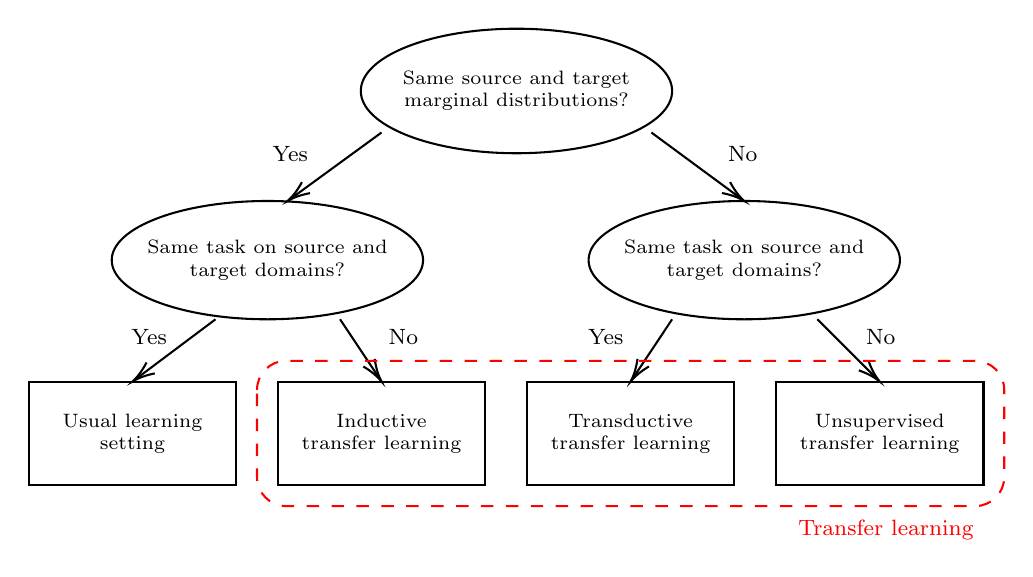
\begin{tikzpicture}[x=0.75pt,y=0.75pt,yscale=-1,xscale=1]
%uncomment if require: \path (0,269); %set diagram left start at 0, and has height of 269

%Shape: Ellipse [id:dp0974795717337551] 
\draw   (160,40) .. controls (160,23.43) and (193.58,10) .. (235,10) .. controls (276.42,10) and (310,23.43) .. (310,40) .. controls (310,56.57) and (276.42,70) .. (235,70) .. controls (193.58,70) and (160,56.57) .. (160,40) -- cycle ;
%Shape: Ellipse [id:dp9862877791048306] 
\draw   (40,121.5) .. controls (40,105.76) and (73.58,93) .. (115,93) .. controls (156.42,93) and (190,105.76) .. (190,121.5) .. controls (190,137.24) and (156.42,150) .. (115,150) .. controls (73.58,150) and (40,137.24) .. (40,121.5) -- cycle ;
%Shape: Ellipse [id:dp314231133167162] 
\draw   (269.75,121.5) .. controls (269.75,105.76) and (303.33,93) .. (344.75,93) .. controls (386.17,93) and (419.75,105.76) .. (419.75,121.5) .. controls (419.75,137.24) and (386.17,150) .. (344.75,150) .. controls (303.33,150) and (269.75,137.24) .. (269.75,121.5) -- cycle ;
%Shape: Rectangle [id:dp9001687557476825] 
\draw   (0,180) -- (100,180) -- (100,230) -- (0,230) -- cycle ;
%Shape: Rectangle [id:dp37462803697884417] 
\draw   (120,180) -- (220,180) -- (220,230) -- (120,230) -- cycle ;
%Shape: Rectangle [id:dp41799431397747233] 
\draw   (240,180) -- (340,180) -- (340,230) -- (240,230) -- cycle ;
%Shape: Rectangle [id:dp7754162600589308] 
\draw   (360,180) -- (460,180) -- (460,230) -- (360,230) -- cycle ;
%Straight Lines [id:da9176701651556409] 
\draw    (170,60) -- (126.37,91.82) ;
\draw [shift={(124.75,93)}, rotate = 323.9] [color={rgb, 255:red, 0; green, 0; blue, 0 }  ][line width=0.75]    (10.93,-3.29) .. controls (6.95,-1.4) and (3.31,-0.3) .. (0,0) .. controls (3.31,0.3) and (6.95,1.4) .. (10.93,3.29)   ;
%Straight Lines [id:da25605932186071767] 
\draw    (300,60) -- (343.14,91.81) ;
\draw [shift={(344.75,93)}, rotate = 216.41] [color={rgb, 255:red, 0; green, 0; blue, 0 }  ][line width=0.75]    (10.93,-3.29) .. controls (6.95,-1.4) and (3.31,-0.3) .. (0,0) .. controls (3.31,0.3) and (6.95,1.4) .. (10.93,3.29)   ;
%Straight Lines [id:da5288229165358177] 
\draw    (90,150) -- (51.6,178.8) ;
\draw [shift={(50,180)}, rotate = 323.13] [color={rgb, 255:red, 0; green, 0; blue, 0 }  ][line width=0.75]    (10.93,-3.29) .. controls (6.95,-1.4) and (3.31,-0.3) .. (0,0) .. controls (3.31,0.3) and (6.95,1.4) .. (10.93,3.29)   ;
%Straight Lines [id:da9359408976926888] 
\draw    (150,150) -- (168.89,178.34) ;
\draw [shift={(170,180)}, rotate = 236.31] [color={rgb, 255:red, 0; green, 0; blue, 0 }  ][line width=0.75]    (10.93,-3.29) .. controls (6.95,-1.4) and (3.31,-0.3) .. (0,0) .. controls (3.31,0.3) and (6.95,1.4) .. (10.93,3.29)   ;
%Straight Lines [id:da3772543817005427] 
\draw    (310,150) -- (291.11,178.34) ;
\draw [shift={(290,180)}, rotate = 303.69] [color={rgb, 255:red, 0; green, 0; blue, 0 }  ][line width=0.75]    (10.93,-3.29) .. controls (6.95,-1.4) and (3.31,-0.3) .. (0,0) .. controls (3.31,0.3) and (6.95,1.4) .. (10.93,3.29)   ;
%Straight Lines [id:da11594261351341528] 
\draw    (380,150) -- (408.59,178.59) ;
\draw [shift={(410,180)}, rotate = 225] [color={rgb, 255:red, 0; green, 0; blue, 0 }  ][line width=0.75]    (10.93,-3.29) .. controls (6.95,-1.4) and (3.31,-0.3) .. (0,0) .. controls (3.31,0.3) and (6.95,1.4) .. (10.93,3.29)   ;
%Rounded Rect [id:dp8619685472332226] 
\draw  [color={rgb, 255:red, 255; green, 0; blue, 0}  ,draw opacity=1 ][dash pattern={on 4.5pt off 4.5pt}] (110,184) .. controls (110,176.27) and (116.27,170) .. (124,170) -- (456,170) .. controls (463.73,170) and (470,176.27) .. (470,184) -- (470,226) .. controls (470,233.73) and (463.73,240) .. (456,240) -- (124,240) .. controls (116.27,240) and (110,233.73) .. (110,226) -- cycle ;
% Text Node
\draw (235,40) node  [font=\scriptsize] [align=center] {
Same source and target\\marginal distributions?
};
% Text Node
\draw (344.75,121.5) node  [font=\scriptsize] [align=center] {
Same task on source and\\target domains?
};
% Text Node
\draw (115,121.5) node  [font=\scriptsize] [align=center] {
Same task on source and\\target domains?
};
% Text Node
\draw (50,205) node  [font=\scriptsize] [align=center] {
Usual learning\\setting
};
% Text Node
\draw (170,205) node  [font=\scriptsize] [align=center] {
Inductive\\transfer learning
};
% Text Node
\draw (290,205) node  [font=\scriptsize] [align=center] {
Transductive\\transfer learning
};
% Text Node
\draw (410,205) node  [font=\scriptsize] [align=center] {
Unsupervised\\transfer learning
};
% Text Node
\draw (126,70.5) node  [font=\footnotesize] [align=left] {Yes};
% Text Node
\draw (344,70.5) node  [font=\footnotesize] [align=left] {No};
% Text Node
\draw (58,158.5) node  [font=\footnotesize] [align=left] {Yes};
% Text Node
\draw (410.5,158.5) node  [font=\footnotesize] [align=left] {No};
% Text Node
\draw (180.5,158.5) node  [font=\footnotesize] [align=left] {No};
% Text Node
\draw (278,158.5) node  [font=\footnotesize] [align=left] {Yes};
% Text Node
\draw (413,251.5) node  [font=\footnotesize,color={rgb, 255:red, 255; green, 0; blue, 0 }  ,opacity=1 ] [align=left] {Transfer learning};
\end{tikzpicture}
\caption{Positioning transfer learning with respect to the typical learning setting. Categories of transfer learning differ either with respect to the marginal distribution. Reproduced from }
\label{fig:transfer_modes}
\end{figure}

Neural networks, with their endless flexibility, are well-equipped for transfer learning. Shortly after the deep learning revolution in 2012 (see Appendix \ref{sec:brief_history_classifiers}), the potential for the learning transfer of powerful pretrained neural networks was discovered (see \cite{zeiler2014visualizing} and \cite{sharif2014cnn}). Pretrained networks are usually used in one of two ways:

\begin{enumerate}
\item feature extraction: a pretrained network is used to extract features for a new problem, by passing images forward through its hidden layers and recording a given layer (``CNN code'') as a vector of (obscure) image features
\item fine-tuning: a pretrained network recommences training on a new problem from the previous point of convergence, usually at a significantly lower learning rate, and often only on the deepest layers.
\end{enumerate}

Both approaches have seen widespread use. Pretraining is usually done on a large standard image corpus like ImageNet. The success of these approaches illustrates the universality of the filters learned by deep networks, as general images. It  For this reason, neither approach fits easily into the schema of Figure \ref{fig:transfer_modes}. If the target images are similar in resolution and content, for example, the low-level neural activity of earlier layers may be identical to the source dataset, resembling inductive transfer learning.

\section{Fighting overfitting in machine learning}

In machine learning, overfitting is the effect of \emph{fitting the noise instead of the signal}. In practice, all data contains noise obscuring the ground signal, and when a dataset is sufficiently small, a modestly powerful model may interpolate it perfectly, only to then be useless on test data. Take for example k-nearest neighbours (kNN), a simple, non-parametric classifier (Figure \ref{fig:knn}). For small $k$, outliers have undue influence on local test data, creating discontinuous decision boundaries, with high resulting test error.

\begin{figure}%
    \centering
    \subfloat[$k = 1$]{{\includegraphics[width=0.45\textwidth]{img/knn1.pdf}}}
    \qquad
    \subfloat[$k = 7$]{{\includegraphics[width=0.45\textwidth]{img/knn7.pdf}}}
	\caption{Visualisation of overfitting with k-nearest neighbours (kNN) (non-parametric model). A data point is classified as the majority class of the $k$ geometrically closest data points. Note the steadier decision boundary formed for $k = 7$. Taken from https://github.com/jcboyd/lastchancestats}
    \label{fig:knn}%
\end{figure}

Much of machine learning is ultimately concerned with striking a balance between overfitting and underfitting. In supervised learning, this balance is evaluated with \emph{generalisation error}, the ability of the model to generalise the data, which is estimated by evaluating a trained model over a test set of independent, unseen data. The \emph{bias-variance decomposition} illustrates the tradeoff between over- and underfitting. Suppose we have $Y = f(x) + \epsilon$ generating training data with $f(x)$ the true signal for data point $x$, and noise, $\epsilon = \mathcal{N}(0, \sigma^2)$. Let our model estimate be denoted by $\hat{f}(x)$. Then, the MSE (here an arbitrary measure of goodness of fit) between an estimate and the true parameters, averaged over all possible data,

\begin{align}
\mathbb{E}[(Y - \hat{f}(x))^2] &= \mathbb{E}[((f(x) + \epsilon - \mathbb{E}[\hat{f}(x)]) + (\mathbb{E}[\hat{f}(x)] - \hat{f}(x)))^2] \\
&= \sigma^2 + \mathbb{E}[f(x) - \mathbb{E}[\hat{f}(x)]]^2 + \mathbb{E}[(\hat{f}(x) - \mathbb{E}[\hat{f}(x)])^2] \\
&= \text{noise} + \text{bias}^2 + \text{variance}
\end{align}

where in step (1.2) some terms are eliminated with zero mean. Note the positive terms means this represents a lower bound on error. The bias term represents underfitting as a simplified model fails to follow a more complex trend (for example a linear model undershooting a higher-order function). This bias will be observed in training error. The variance term represents overfitting as the model varies around its mean greatly to interpolate noisy data. This variance will be observed in test error.

There are various strategies to attenuate overfitting. A common approach is \emph{regularisation}. This usually takes the form of a penalty term. For example, introducing a $l_2$ penalty to a linear regression gives us the ridge regression objective,

\begin{equation}
\min_\beta\mathcal{L} = \frac{1}{2}(\mathbf{y} - \mathbf{X}\boldsymbol\beta)^T(\mathbf{y} - \mathbf{X}\boldsymbol\beta) + \frac{\lambda}{2}\boldsymbol\beta^T\boldsymbol\beta
\end{equation}

for input and target data $(\mathbf{X}, \mathbf{y})$, model parameters $\beta$ and penalty tuning parameter $\lambda$. Complex models that overfit usually require large parameter values (in the extreme, a degree $n$ polynomial with up to $n-1$ turning points can interpolate $n+1$ data points), so regularisation curtails this tendency. 

Deep learning succeeds because it embodies a different type of bias. Between layers of a basic fully-connected network, the number of weights is quadratic in the number of neurons per layer. Deep learning models reduce this dimensionality by spatial weight sharing, in the case of convolutional network, and weight sharing in time, in the case of recurrent neural networks. These may be referred to as \emph{structural biases}.

%\begin{figure}
%\centering
%\begin{tabular}{cc}
%\subfloat[$k = 1$]{\includegraphics[width=0.5\textwidth]{Figures/knn1.pdf}} & 
%\subfloat[$k = 7$]{\includegraphics[width=0.5\textwidth]{Figures/knn7.pdf}}
%\end{tabular}
%\caption{Visualisation of overfitting with k-nearest neighbours (kNN) (non-parametric model). A data point is classified as the majority class of the $k$ geometrically closest data points. Note the steadier decision boundary formed for $k = 7$. This classifier can be very effective, but suffers from the curse of dimensionality. Data normalisation and dimensionality reduction usually help. However, in certain high-dimensional data sets where data is confined to a lower-dimensional manifold, for example in OCR data, kNN can be very effective. Unlike most classifiers, test time is much greater than training time. Approximations using memory tradeoffs mitigate this. Created with \texttt{knnDemo.m}.}
%\label{fig:knn}
%\end{figure}

\subsection{Data augmentation}

In the long run, as more data is added, a model with sufficient capacity improves its predictive power (generalisation error). In an ideal world, our data is unlimited. However, annotated data for supervised training is expensive, requiring manual effort, often by domain experts. Data augmentation is a technique for obtaining new data fighting overfitting in machine learning models thereby improving generalisation (test time) error (\cite{shorten2019survey}). The idea is to extract additional data \emph{gratis} from the available dataset, by means of bootstrapping or interpolation. A classic algorithm is SMOTE (Synthetic Minority Over-sampling TechniquE) (\cite{chawla2002smote}), which interpolates lines between training samples and their nearest neighbours in feature space, to create synthetic points, and as an alternative to over-sampling by replacement.

Data augmentation is especially vital in deep learning, where powerful neural networks require large datasets to train. Due to the geometry of natural images (pixels are ordered and neighbouring pixels are highly correlated), image data is uniquely receptive to data augmentation, and humans are well-equipped for the engineering of it. Images support a multitude of \emph{label-preserving transformations}, that is, transformations of lower-level image properties that nevertheless maintain the high-level semantic content. Examples are cropping, flipping, rotating, noise injection, convolution, and colour space transformations (if colour is available). These may be referred to as basic image manipulations (\cite{shorten2019survey}) and be ``stacked'' (combined) endlessly, especially on the fly during training. Classic examples include image warping \cite{lecun1998gradient}, elastic deformations \cite{simard2003best}, and PCA-based colour space transformation \cite{krizhevsky2012imagenet}. However, data augmentation must not be mistaken as equivalent to adding authentic and may reinforce existing biases in a dataset (\cite{shorten2019survey}). The augmented images are highly interdependent and will not in general amount to substantially increasing the coverage of the image space (see Figure \ref{fig:augmentation}). Additionally, certain transformations will be domain-specific. For example, biomedical imagery can usually be rotated arbitrarily without losing meaning, unlike images of everyday objects or handwritten digits.

\begin{figure}[h]
\centering

\tikzset{every picture/.style={line width=0.75pt}} %set default line width to 0.75pt        

\begin{tikzpicture}[x=0.75pt,y=0.75pt,yscale=-1,xscale=1]
%uncomment if require: \path (0,267); %set diagram left start at 0, and has height of 267

%Image [id:dp4690746643617628] 
\draw (305,135) node  {\includegraphics[width=37.5pt,height=37.5pt]{img/augmentation_cat_aug2.png}};
%Shape: Rectangle [id:dp5844515089762182] 
\draw   (280,110) -- (330,110) -- (330,160) -- (280,160) -- cycle ;

%Image [id:dp8031263564437391] 
\draw (215,175) node  {\includegraphics[width=37.5pt,height=37.5pt]{img/augmentation_cat.png}};
%Shape: Rectangle [id:dp007056558703781413] 
\draw   (190,150) -- (240,150) -- (240,200) -- (190,200) -- cycle ;

%Image [id:dp08461336687255161] 
\draw (115,95) node  {\includegraphics[width=37.5pt,height=37.5pt]{img/augmentation_deer.png}};
%Shape: Rectangle [id:dp6749055875742906] 
\draw   (90,70) -- (140,70) -- (140,120) -- (90,120) -- cycle ;

%Image [id:dp464239246082056] 
\draw (435,115) node  {\includegraphics[width=37.5pt,height=37.5pt]{img/augmentation_truck.png}};
%Shape: Rectangle [id:dp39795630279129157] 
\draw   (410,90) -- (460,90) -- (460,140) -- (410,140) -- cycle ;

%Image [id:dp24631782250209233] 
\draw (395,175) node  {\includegraphics[width=37.5pt,height=37.5pt]{img/augmentation_car.png}};
%Shape: Rectangle [id:dp6628152059484871] 
\draw   (370,150) -- (420,150) -- (420,200) -- (370,200) -- cycle ;

%Image [id:dp8576511044757406] 
\draw (65,155) node  {\includegraphics[width=37.5pt,height=37.5pt]{img/augmentation_horse.png}};
%Shape: Rectangle [id:dp827131947184459] 
\draw   (40,130) -- (90,130) -- (90,180) -- (40,180) -- cycle ;

%Image [id:dp9366678348308388] 
\draw (265,75) node  {\includegraphics[width=37.5pt,height=37.5pt]{img/augmentation_cat_aug1.png}};
%Shape: Rectangle [id:dp2003057013901418] 
\draw   (240,50) -- (290,50) -- (290,100) -- (240,100) -- cycle ;

%Shape: Sine Wave Form [id:dp44457004411395107] 
\draw   (20,139.57) .. controls (113.59,0.73) and (157.72,0) .. (249.97,139.57) .. controls (342.28,279.14) and (385.54,280) .. (480,139.57) ;
%Shape: Circle [id:dp6762877746787627] 
\draw  [fill={rgb, 255:red, 208; green, 2; blue, 27 }  ,fill opacity=1 ] (34,112) .. controls (34,108.69) and (36.69,106) .. (40,106) .. controls (43.31,106) and (46,108.69) .. (46,112) .. controls (46,115.31) and (43.31,118) .. (40,118) .. controls (36.69,118) and (34,115.31) .. (34,112) -- cycle ;
%Shape: Circle [id:dp8216805850204476] 
\draw  [fill={rgb, 255:red, 208; green, 2; blue, 27 }  ,fill opacity=1 ] (68,70) .. controls (68,66.69) and (70.69,64) .. (74,64) .. controls (77.31,64) and (80,66.69) .. (80,70) .. controls (80,73.31) and (77.31,76) .. (74,76) .. controls (70.69,76) and (68,73.31) .. (68,70) -- cycle ;
%Shape: Circle [id:dp5289135761245862] 
\draw  [fill={rgb, 255:red, 208; green, 2; blue, 27 }  ,fill opacity=1 ] (244.97,140.57) .. controls (244.97,137.26) and (247.66,134.57) .. (250.97,134.57) .. controls (254.28,134.57) and (256.97,137.26) .. (256.97,140.57) .. controls (256.97,143.88) and (254.28,146.57) .. (250.97,146.57) .. controls (247.66,146.57) and (244.97,143.88) .. (244.97,140.57) -- cycle ;
%Shape: Circle [id:dp5124108509736214] 
\draw  [fill={rgb, 255:red, 74; green, 144; blue, 226 }  ,fill opacity=1 ] (233,122) .. controls (233,118.69) and (235.69,116) .. (239,116) .. controls (242.31,116) and (245,118.69) .. (245,122) .. controls (245,125.31) and (242.31,128) .. (239,128) .. controls (235.69,128) and (233,125.31) .. (233,122) -- cycle ;
%Shape: Circle [id:dp3304180493841744] 
\draw  [fill={rgb, 255:red, 74; green, 144; blue, 226 }  ,fill opacity=1 ] (257,159) .. controls (257,155.69) and (259.69,153) .. (263,153) .. controls (266.31,153) and (269,155.69) .. (269,159) .. controls (269,162.31) and (266.31,165) .. (263,165) .. controls (259.69,165) and (257,162.31) .. (257,159) -- cycle ;
%Shape: Circle [id:dp5055457984695153] 
\draw  [fill={rgb, 255:red, 208; green, 2; blue, 27 }  ,fill opacity=1 ] (426,204) .. controls (426,200.69) and (428.69,198) .. (432,198) .. controls (435.31,198) and (438,200.69) .. (438,204) .. controls (438,207.31) and (435.31,210) .. (432,210) .. controls (428.69,210) and (426,207.31) .. (426,204) -- cycle ;
%Shape: Circle [id:dp11055235341340652] 
\draw  [fill={rgb, 255:red, 208; green, 2; blue, 27 }  ,fill opacity=1 ] (455,167) .. controls (455,163.69) and (457.69,161) .. (461,161) .. controls (464.31,161) and (467,163.69) .. (467,167) .. controls (467,170.31) and (464.31,173) .. (461,173) .. controls (457.69,173) and (455,170.31) .. (455,167) -- cycle ;
\end{tikzpicture}
\caption{Data augmentation can make modest but useful interpolations of the space surrounding real images. CIFAR-10 images marked by red circle; augmented images marked by blue circle; black line represents natural image manifold. Upper augmentation based on conversion to grayscale (an element-wise weighted average of the RGB pixels) and rotation; the lower on colour inversion and horizontal flipping.}
\label{fig:augmentation}
\end{figure}

Deep learning is a powerful albeit more expensive for data augmentation. One good example is \emph{adversarial training}. \cite{goodfellow2014explaining} show how with a precise perturbation to a model input, one may ``fool'' a linear model or neural network alike. Consider perturbing model input $\mathbf{x}$,

\begin{equation}
\hat{\mathbf{x}} = \mathbf{x} + \alpha\cdot\eta,
\end{equation}

where $\eta = \text{sign}(\mathbf{w})$ for $\mathbf{w}$ are the model weights of a softmax regression model and $\alpha$ a tuning parameter. Now, the model will predict $\sigma(\mathbf{w}^T\hat{\mathbf{x}}) = \sigma(\mathbf{w}^T\mathbf{x} + \alpha\cdot||\mathbf{w}||_1)$. If $\mathbf{x}$ is sufficiently high-dimensional (as image data often is) the perturbations will accumulate even for $\alpha << 1$ and can change the decision of the model. This produces a paradox especially apparent for image data: one may, for example, add a small, carefully chosen value to each pixel of an image, and the model may suddenly predict the wrong object class with high confidence, even though the perturbation is imperceptible to the human eye. This paradox defies intuitions about how neural networks represent images and ``adversarial attacks'' remain problematic for deep learning. \cite{goodfellow2014explaining} nevertheless showed how adversarial attacks could be harnessed during training to strengthen neural networks against such attacks, in effect a sort of data augmentation.

Generative models, in particular generative adversarial models (GANs) (\cite{goodfellow2014generative}) (loosely related to the above) are a more recent and exciting prospect for data augmentation. Generative models are trained to learn (perhaps implicitly) the data-generating distribution, and thereupon may be used as a sampling system for synthetic data. Ideally, a generative model based on deep neural networks will make for a more powerful interpolation system than any of the above.

One may also consider transfer learning as a form of data augmentation commuted via pretrained model. The information content of a rich source dataset $\mathcal{D}_S$ may be distilled by a powerful neural network, and transferred to augment the available data for learning some task on a target dataset $\mathcal{D}_T$. Indeed, style transfer involving deep, pretrained networks \cite{gatys2016image} is a powerful mode of data augmentation, as we discover in Chapter \ref{Chapter5}.

%\section{Adversarial methods}
%
%The work of \cite{karras2017progressive} is truly impressive. The authors propose a training strategy for taking GANs to high resolution (up to $1024^2$ pixels). Training is done in stages, beginning at low resolutions ($4\times 4$), and increasing the resolution twofold at intervals. This is done simply by adding new layers to the generator and discriminator, which remain symmetric throughout training. To curtail the impact of adding new layers with random weights, the new layer is ``faded in'' with a residual collection, allowing it to simply perform the identity operation at first, before the skip connection is gradually turned off\footnote{This highlights the power of the residual block for facilitating learning in deep networks.}. Thus, the GAN learns global structures first at low resolution, and progressively refines its output. They find that this approach makes for faster learning than comparable approaches, which otherwise attempt to learn all structure (global and fine) at once. Note this is not a greedy optimisation, as all layers remain trainable throughout; the authors describe it rather as implicit curriculum learning (i.e. learning easy tasks first before ramping difficulty up).
